\documentclass[11pt]{article}
\usepackage[utf8]{inputenc}
\usepackage[T1]{fontenc}
\usepackage[french]{babel}
\usepackage{amsmath,amssymb,amsthm}
\usepackage{booktabs}
\usepackage{array}
\newcolumntype{L}[1]{>{\raggedright\arraybackslash}p{#1}}
\usepackage{graphicx}
% ---------------------------------------------------------------------------
% LISIBILITE — docs/articles/STYLE_ARTICLES.md §2.
% ---------------------------------------------------------------------------
\usepackage[a4paper,textwidth=13.8cm,textheight=22.4cm]{geometry}
\linespread{1.06}
\setlength{\parskip}{.55em plus .15em minus .1em}
\setlength{\parindent}{1.1em}
\emergencystretch=1.5em
\usepackage{hyperref}

% ============================================================================
% TRADUCTION de main.tex. Toute correction de FOND se fait dans l'anglais
% d'abord, puis se reporte ici. Les chiffres viennent de MESURES.md.
% ============================================================================

\newtheorem{definition}{Définition}
\newtheorem{proposition}{Proposition}
\theoremstyle{remark}\newtheorem{remarque}{Remarque}

\title{La marche du dernier kilomètre~:\\
une recherche gardée par le noyau, qui invente ses propres relais}

\author{Karl Olivet\thanks{Chercheur indépendant. Contact~:
\texttt{karl.olivet@gmail.com}. Code et corpus certifié~:
\url{https://github.com/Karl-O/bourbaki-theorie-des-ensembles}~; chaque
chiffre rapporté ici a été mesuré le 21 août 2026 et consigné, avec son
expérience, dans \texttt{article/marcheur/MESURES.md}.}}

\date{Préprint --- août 2026\\
{\small Traduction française de travail --- la version de référence est l'anglaise (\texttt{main.tex}).}}

\begin{document}
\maketitle

\begin{abstract}
Un article compagnon soutenait qu'en recherche de preuve mécanisée le dernier
kilomètre se localise, il ne se franchit pas~: une recherche qui échoue doit
nommer exactement ce qui lui manque. Cet article rapporte l'étape suivante ---
un \emph{marcheur} qui traverse le tronçon que le système précédent savait
seulement localiser. Devant un but que le chaînage arrière seul ne ferme pas
--- mesuré~: sur une réassociation à quatre éléments d'une opération dérivée
$a \oplus b := (a+b)+1$, le chaînage épuise son budget en 692\,s --- le
marcheur mine les sous-termes du but à la recherche de motifs répétés,
redécouvre $\oplus$ sans qu'on lui dise qu'il existe, conjecture ses lois sur
une liste ouverte de schémas, laisse un oracle numérique tuer les fausses en
quelques millisecondes, fait certifier les vraies par le noyau, et re-essaie
le but sur le pool \emph{comprimé} des seuls lemmes dérivés. Le même but se
ferme alors, contrôlé par le noyau, en 414\,s de bout en bout --- moins de
temps qu'il n'en faut au chaînage pour échouer. Deux faits mesurés encadrent
la contribution. D'abord, la compression est un \emph{remplacement}, pas un
ajout~: re-essayer sur le seul lemme dérivé prend 72,6\,s, l'ajouter aux lois
brutes en prend 962 --- un facteur 13, parce qu'un savoir nouveau agrandit
l'espace de recherche tant que l'ancien n'est pas mis de côté. Ensuite, le
premier composant du marcheur a échoué d'une façon qui mérite d'être
rapportée~: classer les motifs candidats par taille ne sélectionnait que des
fragments des énormes développements $\tau$ (un terme à trois $\oplus$ fait
$\approx$13\,700 nœuds) et manquait $\oplus$ entièrement~; le remède ---
apparier les sous-termes par signature de racine --- est lui-même une loi de
conception mesurée. Comme partout dans cette série, le noyau garde chaque
pas~: une mauvaise proposition coûte une route morte, jamais un faux
théorème.
\end{abstract}

%% ============================================================================
\section{Introduction}
\label{sec:intro}
%% ============================================================================

L'article compagnon sur le compte rendu d'échec se terminait sur une porte
qu'il refusait de franchir~: son plan éditorial exige qu'aucun marcheur ne
soit publié avant d'avoir fermé au moins un but que le chaînage seul ne ferme
pas. Cet article commence par franchir cette porte, mesurée des deux côtés,
et tout le reste en découle.

\paragraph{La revendication, en un paragraphe.} Un but qui met en échec une
recherche arrière bornée ne la met généralement pas en échec par la seule
profondeur. Ce qui manque est un \emph{relais}~: un énoncé intermédiaire qui,
une fois certifié et versé au pool, rend courte la distance restante. Le
travail du marcheur est d'inventer des relais candidats depuis la structure
même du but, d'écarter les faux à bas prix, de payer au noyau le prix des
vrais, puis d'attaquer le but depuis le relais plutôt que depuis les lois
brutes. Rien de tout cela n'exige que la machine ait raison~: chaque candidat
est jugé --- d'abord par un oracle numérique qui ne sait que réfuter, puis
par le noyau qui seul sait certifier. Une proposition fausse coûte des
secondes~; une proposition non sûre est impossible.

\paragraph{Contributions.} Tous les chiffres ont été mesurés le 21 août 2026
et sont reproductibles depuis le dépôt (section~\ref{sec:repro}).
\begin{itemize}
\item \textbf{La porte, franchie et assertée des deux côtés}
  (sections~\ref{sec:porte} et~\ref{sec:marche})~: le chaînage seul échoue
  sur $B_4$ en 692\,s~; un appel au marcheur, sans surveillance, le ferme,
  contrôlé noyau, en 414\,s. Un test du dépôt asserte les deux côtés.
\item \textbf{Remplacement, pas ajout, mesuré trois fois}
  (sections~\ref{sec:porte} et~\ref{sec:marche})~: le lemme dérivé seul,
  72,6\,s~; avec un lemme vrai de plus, 361\,s~; ajouté aux lois brutes,
  962\,s~; les six lemmes certifiés d'un coup, plus de 580\,s puis tué.
  D'où l'échelle de compression du marcheur.
\item \textbf{Un mineur qui redécouvre l'opération depuis le but}
  (section~\ref{sec:mineur}) --- y compris l'échec mesuré de sa première
  version, qui classait par taille et ne voyait que le bruit des
  développements $\tau$.
\item \textbf{Un oracle de réfutation à l'angle mort déclaré}
  (section~\ref{sec:oracle})~: une couche ajoutée rend visibles les
  conjectures sur opérations dérivées~; ce qui reste invisible a coûté
  11\,s mesurées d'échecs de certification sur ce banc.
\end{itemize}

%% ============================================================================
\section{Cadre~: le banc, le budget, le manque}
\label{sec:background}
%% ============================================================================

Nous reprenons le banc d'algèbre jouet sur lequel l'article compagnon a
mesuré ses organes de réécriture. La théorie de base fournit l'addition
cardinale $a+b$ et ses deux lois brutes --- associativité itérée et
commutativité --- comme seuls faits du pool. Par-dessus, une opération
dérivée est définie et n'est nommée nulle part dans le dépôt~:
\[
a \oplus b \;:=\; (a+b)+1 .
\]
Le budget du moteur n'est pas une estimation~: la chaîne de réécriture brute
minimale pour l'associativité à trois éléments de $\oplus$ a été mesurée à
cinq pas, et cinq est donc le plafond du moteur (\texttt{max\_pas=5})~; avec
un plafond de trois, ce même but échouait. Toutes les expériences ci-dessous
héritent de ce budget mesuré.

Le but qui franchit la porte est la réassociation à quatre éléments
\[
B_4 \;:\;\; ((a \oplus b) \oplus c) \oplus d \;=\; a \oplus (b \oplus (c
\oplus d)),
\]
vraie, et hors de portée d'une chaîne brute de cinq pas~: chaque application
de l'associativité de $\oplus$ coûte environ cinq pas bruts, et $B_4$ en
demande deux.

%% ============================================================================
\section{La porte, mesurée des deux côtés}
\label{sec:porte}
%% ============================================================================

\begin{center}\small
\begin{tabular}{@{}L{0.42\linewidth}L{0.24\linewidth}r@{}}
\toprule
expérience & verdict & durée \\
\midrule
chaînage seul sur $B_4$ (pool brut) & \textbf{échoue}, un manque nommé & 692,5\,s \\
certification du lemme $\oplus$-assoc & fermé, contrôlé noyau & 4--7\,s \\
$B_4$ sur le pool \emph{comprimé} (lemme seul) & \textbf{fermé}, 0 hypothèse & 72,6\,s \\
$B_4$ sur le pool cumulé (brut $+$ lemme) & fermé & 962,4\,s \\
variante fausse $F_4$ sur le pool comprimé & reste ouverte (bien) & 79,1\,s \\
\bottomrule
\end{tabular}
\end{center}

Trois lectures, par importance décroissante.

\paragraph{La porte tient.} Le même but, depuis le même pool, sous les mêmes
budgets~: le chaînage s'épuise en 692\,s et rend un manque nommé~; la marche
en deux pas --- certifier le relais, puis re-essayer depuis lui --- le ferme.
« Ne ferme pas » n'est pas ici une affirmation asymptotique~; c'est le
comportement mesuré du moteur complet à 21 organes, à son budget mesuré.

\paragraph{La compression est un remplacement, pas un ajout.} Le chiffre le
plus utile du tableau est le moins intuitif~: ajouter le lemme certifié aux
lois brutes rend la recherche \emph{treize fois plus lente} que les remplacer
par lui (962\,s contre 72,6\,s). Chaque fait du pool est un candidat de
réécriture à chaque nœud~; un savoir nouveau agrandit l'espace tant que
l'ancien n'est pas mis de côté. Le marcheur re-essaie donc ses buts sur les
seuls lemmes dérivés --- et le dit dans son journal, jamais en silence.

\paragraph{Le coût de certification est bruité.} Le même lemme certifié deux
fois a pris 3,8\,s puis 7,4\,s selon l'état des caches. Nous citons
« quelques secondes » et refusons un chiffre unique.

%% ============================================================================
\section{Le marcheur}
\label{sec:marcheur}
%% ============================================================================

L'état du marcheur est un couple (but, pool de faits certifiés). Un pas~:

\begin{enumerate}
\item \textbf{Sentir.} Lancer l'organe de besoin. Fermé~: fini. Ouvert~: une
  liste de manques nommés --- l'objet d'échec de l'article compagnon.
\item \textbf{Miner.} Extraire du but lui-même ses motifs de termes répétés,
  par anti-unification à slots partagés, classés par le gain MDL
  $(\mathrm{occurrences}-1) \times \mathrm{taille}$ --- le critère de
  compression de l'organe mineur de notions, transposé des formules aux
  termes.
\item \textbf{Conjecturer.} Instancier les schémas de lois sur chaque motif
  binaire~: commutativité, associativité, idempotence. La liste des schémas
  est \emph{ouverte}~; rien ne prouve que ces trois suffisent, et l'article
  ne le revendique pas.
\item \textbf{Réfuter à bas prix.} Un oracle numérique cherche de petits
  contre-exemples. Une conjecture fausse meurt en millisecondes, jamais en
  minutes de noyau. L'oracle ne sait que réfuter~: l'absence de
  contre-exemple autorise la dépense, et ne prouve rien.
\item \textbf{Certifier, comprimer, re-essayer.} Les conjectures survivantes
  passent à l'organe de besoin sur le pool brut~; le noyau juge. Les lemmes
  certifiés forment le pool comprimé sur lequel le but est re-essayé. Aucun
  progrès dans une ronde~: s'arrêter, et rendre les manques terminaux --- le
  marcheur, comme l'organe qu'il enveloppe, échoue en nommant.
\end{enumerate}

Le principe de sûreté est inchangé depuis le premier organe proposeur~: le
marcheur \emph{suggère}, le noyau \emph{juge}. Aucun objet théorème n'est
construit dans le code du marcheur~; tout ce qui entre au pool est sorti de
l'organe de besoin, donc du noyau.

%% ============================================================================
\section{Le mineur, y compris son premier échec}
\label{sec:mineur}
%% ============================================================================

Le mineur répond à la question que le lecteur doit se poser~: \emph{qui a
parlé de $\oplus$ à la machine~?} Personne. Le motif est retrouvé dans le
but.

\paragraph{La version 1 a échoué, et cet échec est une loi de conception.}
Le premier mineur collectait les sous-termes du but et anti-unifiait les 24
plus gros. Il n'a rien trouvé d'utilisable~: dans ce noyau les termes sont
des développements $\tau$ opaques, un terme à trois $\oplus$ fait
${\approx}13\,700$ nœuds, si bien que les plus gros sous-termes sont tous des
\emph{fragments de l'intérieur des développements} --- et les petites
instances $a \oplus b$, celles qui portent le motif, n'entraient jamais dans
le top-24. Le motif de tête était un contexte à trois slots de gain MDL
13\,737, inutilisable pour conjecturer, et $\oplus$ était absent de la liste.
Classer par taille sélectionne le bruit.

\paragraph{La version 2 apparie par signature de racine.} Les sous-termes
sont groupés par signature de racine (tag, nom, lieur, arité) et chacun est
anti-unifié avec ses voisins de taille \emph{dans son groupe}~: $O(n)$ paires
au lieu de $O(n^2)$, et deux instances d'une même opération se rencontrent
forcément. Les occurrences se comptent ensuite sur \emph{tous} les
sous-termes, et les candidats sont validés par reconstruction~: un motif
appliqué aux morceaux de son propre générateur doit le rebâtir à l'identique
--- les assemblages sont hachables, c'est donc une égalité $O(1)$, jamais une
devinette structurelle. Sur $B_4$ le motif de tête sort avec 6 occurrences et
un gain de 4\,045, et son application à $(a,b)$ donne exactement
$\oplus(a,b)$~: le minage a pris 1,1\,s.

%% ============================================================================
\section{L'oracle avait un trou, une couche a suffi}
\label{sec:oracle}
%% ============================================================================

Le pas de réfutation a mis au jour un angle mort mesuré. L'oracle évalue les
termes par une table de reconstruction --- les numéraux, leurs sommes, leurs
produits --- parce que les termes sont ici opaques~: il n'y a rien où
descendre. Mais --- en notant $\mathrm{succ}$ l'opération successeur, le
$+1$ du $\oplus$ du banc --- $\mathrm{succ}(\text{somme})$ n'était dans
aucune entrée, si bien que \emph{toute} conjecture sur une opération dérivée s'évaluait en
« inconnu »~: invisible, ni réfutable ni autorisée.

Une couche a suffi~: pour chaque terme déjà en table de valeur $v$, ajouter
son successeur avec la valeur $v+1$. Après l'extension, le schéma
d'idempotence de $\oplus$ --- faux --- meurt en moins d'une milliseconde,
avant tout appel noyau~; commutativité et associativité survivent au balayage
(environ une seconde chacune) et passent à la certification. La limite est
dite là où vit le code~: une couche seulement. Un terme dérivé imbriqué comme
$\mathrm{succ}(\mathrm{succ}(a+b)+c)$ reste hors table, la clôture complète
coûterait $|\text{table}|^2$, et sur de telles conjectures l'oracle se tait
--- il n'affirme jamais.

%% ============================================================================
\section{La marche, de bout en bout}
\label{sec:marche}
%% ============================================================================

Tout ce qui précède décrivait des organes~; cette section rapporte la machine
qui les exécute sans surveillance. Un appel --- \texttt{marcher($B_4$, pool
brut)} --- avec une sonde horodatée sur son journal~:

\begin{center}\small
\begin{tabular}{@{}L{0.58\linewidth}rr@{}}
\toprule
phase & fenêtre & durée \\
\midrule
minage (4 motifs, gains 4045/1771/1155/895) & 0--4,0\,s & 4,0\,s \\
12 conjectures~: 6 certifiées, 2 réfutées, 4 échouées & 4,0--53,2\,s & 49,2\,s \\
\quad $\oplus$-commutativité certifiée & & 20,2\,s \\
\quad $\oplus$-associativité certifiée & & 16,8\,s \\
\quad idempotence réfutée (en $x=0$, resp.\ $x=1$) & & ${<}0,1$\,s \\
re-essai, palier 1 de l'échelle (les 2 lemmes du motif de tête) & 53,2--414,2\,s & 361,0\,s \\
\midrule
\textbf{fermé} --- contrôlé noyau, 0 hypothèse, 22 axiomes & & \textbf{414,2\,s} \\
\bottomrule
\end{tabular}
\end{center}

La marche ferme en 414\,s un but que le chaînage passe 692\,s à \emph{ne pas}
fermer. La figure~\ref{fig:chronologie} met côte à côte les quatre recherches
de cet article. Mais le chiffre qui vaut la section est la façon dont le
re-essai a pris sa forme.

\begin{figure}[htbp]
\centering
\resizebox{\ifdim\width>\linewidth \linewidth\else\width\fi}{!}{%
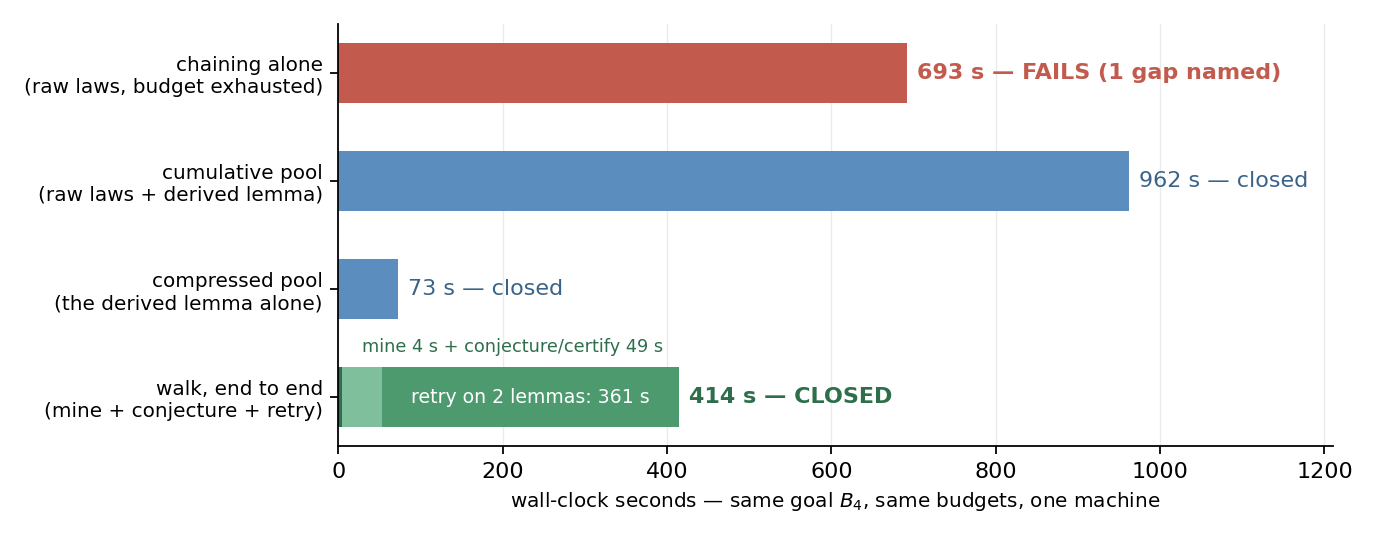
\includegraphics{chronologie.png}}
\caption{Quatre recherches sur le même but $B_4$, mêmes budgets, une machine
(script~: \texttt{scripts/gen\_chronologie.py}, chiffres de
\texttt{MESURES.md}). Le chaînage seul épuise son budget et échoue~; la
marche ferme, et l'essentiel de son temps est le re-essai final --- sur les
deux lemmes du motif de tête seulement. La figure ne prouve aucune
généralité~: un but, un banc, et les durées d'échec dépendent des plafonds
de budget mesurés.}
\label{fig:chronologie}
\end{figure}

\paragraph{La marche a d'abord échoué par sa propre richesse.} La première
version re-essayait le but sur \emph{tous} les lemmes certifiés à la fois ---
six, car les motifs secondaires du mineur donnent eux aussi des lois
certifiables. Ce re-essai a dépassé 580\,s et a été tué~: le marcheur avait
fait de son pool son propre obstacle, exactement la signature « échouer en
grossissant » que l'article compagnon documente pour la recherche brute. Le
remède est l'\emph{échelle de compression}~: re-essayer sur les seuls lemmes
du motif de tête, n'élargir au motif suivant qu'en cas d'échec. Le palier 1 a
suffi. Et une mesure plus fine aiguise la loi du remplacement~: les deux
lemmes du palier ($\oplus$-comm $+$ $\oplus$-assoc) ferment $B_4$ en 361\,s,
quand $\oplus$-assoc \emph{seul} le ferme en 72,6\,s --- même un lemme vrai,
pertinent et certifié de trop coûte un facteur cinq.

\paragraph{Le prix de l'angle mort de l'oracle, mesuré.} Quatre conjectures
(associativité et idempotence des deux motifs secondaires) étaient hors du
fragment de l'oracle à une couche, sont allées à la certification, et y ont
échoué --- environ 11\,s sur les 414. C'est ce que coûte, sur ce banc, la
limite déclarée de la section~\ref{sec:oracle}~: réel, petit, et au journal
plutôt que caché.

\paragraph{Le garde-fou, et ce qu'il a coûté.} La même marche a été pointée
sur une variante fausse $F_4$ (un $d$ là où il faudrait un $c$). Elle a
certifié les mêmes lemmes --- les lemmes parlent de $\oplus$, pas du but ---
puis a échoué honnêtement au premier palier de l'échelle~: 788\,s
d'épuisement, un manque terminal nommé, rien de fermé. Le noyau rend triviale
la moitié forte de cette garantie (aucun faux théorème n'est
\emph{possible})~; ce que l'exécution ajoute est la moitié faible --- le
marcheur ne boucle pas sans fin et ne prétend rien.

Puis la réserve honnête. Sur les paliers supérieurs (pools de quatre à six
lemmes), l'exécution du garde-fou est morte trois fois --- silencieusement~:
ni code de sortie, ni traceback, ni événement système~; cause non identifiée,
corrélée à la taille du pool, pas à la durée. Le test garde-fou du dépôt
plafonne donc l'échelle à un palier \emph{et asserte que le journal le dit}
--- le plafond est un contournement déclaré, pas une optimisation cachée.
Une marche qui échoue et doit gravir toute l'échelle est chère par
construction~; à quel point, nous ne savons pas encore le mesurer jusqu'au
bout.

%% ============================================================================
\section{Ce que la marche ne trouve pas}
\label{sec:limites-goldbach}
%% ============================================================================

Pointé sur l'énoncé général de Goldbach --- le but formalisé en $\tau$ de
l'article compagnon sur la cartographie de l'ouvert, avec les deux mêmes
lois brutes au pool --- le marcheur a fait tout ce que cet article décrit.
Il a miné quatre motifs dans l'énoncé (celui de tête, 8 occurrences, est
la somme dont $2n = p+q$ est fait)~; il a \emph{certifié} des lemmes de
commutativité et d'associativité --- vrais, contrôlés noyau, et portant
sur l'\emph{addition} de l'énoncé, pas sur la primalité~; il a réfuté
deux schémas d'idempotence en $x=1$ et $x=2$~; il a re-essayé sur son
échelle~; et il s'est arrêté sur un état \textbf{terminal en 35,7\,s}, un manque nommé,
rien de fermé, 22 axiomes comme toujours.

C'est la revendication négative de l'article, et sa frontière. La marche ne
crée aucune information mathématique~: des lemmes vrais et certifiés sur
les opérations qu'une conjecture mentionne ne déplacent pas la conjecture.
Le marcheur traverse les derniers kilomètres \emph{pavables} --- fermables
par des lemmes de la théorie qu'il tient déjà~; devant une conjecture
ouverte il fait la seule chose honnête qu'il sache~: s'arrêter vite, et
dire où. Ce que la machine peut dire \emph{du} manque lui-même --- le
reformuler en propriétés d'un $\tau$-terme --- est le sujet de l'article
compagnon, pas de celui-ci.

%% ============================================================================
\section{Reproductibilité}
\label{sec:repro}
%% ============================================================================

Chaque chiffre de cet article a été mesuré le 21 août 2026 et consigné, avec
son expérience, dans \texttt{article/marcheur/MESURES.md}~; les scripts
d'expérience sont versionnés à côté, dans \texttt{article/marcheur/scripts/}
(\texttt{exp1\_porte\_directe.py}, \texttt{exp3\_pool\_comprime.py},
\texttt{exp4\_marche.py}). La porte elle-même est verrouillée par des tests
dans \texttt{outils\_ia/decouvertes/autonomie/test\_general.py}~: un rapide
qui asserte que le mineur redécouvre $\oplus$ et les verdicts de l'oracle, et
deux lents qui assertent les deux côtés de la porte et le garde-fou de la
variante fausse. Les durées sont du temps mural d'appel entier sur une
machine (Python 3.13, Windows)~; la variance de certification de la
section~\ref{sec:porte} s'applique partout.

Les verdicts, lus sur la dernière ligne des fichiers de sortie, jamais sur
une notification~: le test rapide du mineur, 	extbf{1 passed en 34,0\,s}~;
les deux tests lents --- les deux côtés de la porte, et le garde-fou
plafonné --- 	extbf{2 passed en 2673,1\,s} (44\,min\,33).

%% ============================================================================
\section{Travaux voisins}
\label{sec:related}
%% ============================================================================

\paragraph{Exploration de théorie.} Le plus proche parent de la boucle
miner--conjecturer--réfuter--certifier est l'exploration de théorie telle que
la pratique Hipster dans Isabelle/HOL~\cite{johansson2014hipster}, dans la
lignée de QuickSpec~: énumérer des lemmes candidats sur des opérations
données, les filtrer par le test, prouver les survivants. Deux différences
comptent ici. Hipster explore \emph{autour d'une théorie} --- son entrée est
un ensemble d'opérations, sa sortie une bibliothèque~; le marcheur est
\emph{dirigé par le but} --- son entrée est un but unique qu'il doit fermer,
les opérations ne sont pas données mais minées dans les sous-termes de ce
but, et une conjecture n'est certifiée que parce qu'une traversée en a
besoin. Et notre cadre est un calcul du $\tau$ de Bourbaki sur noyau LCF, où
les termes sont des développements opaques~: le pas de minage (et son échec
mesuré) n'a pas d'équivalent quand les termes sont des arbres lisibles. Le
panorama des travaux de conjecture automatique est dressé
par~\cite{conjecturingsurvey2026}.

\paragraph{Le contre-exemple avant la preuve.} Tuer les conjectures par
petits modèles avant de tenter la preuve est une pratique installée
d'Isabelle --- Nitpick et son intégration à
Sledgehammer~\cite{blanchette2011nitpick}~; des travaux récents apprennent à
engendrer des contre-exemples formels par modèles de
langue~\cite{learningtodisprove2026}. Notre oracle est volontairement plus
humble~: une table de reconstruction sur les numéraux, étendue d'une couche
mesurée, dont les angles morts sont déclarés plutôt que lissés --- et dont
les verdicts sont asymétriques par construction, la réfutation certaine, le
silence sinon.

\paragraph{Apprentissage de bibliothèque et compression.} Le critère MDL par
lequel le mineur classe --- nommer ce qui se répète, pondéré par ce que le
nom économise --- est le principe de compression de l'apprentissage de
bibliothèque wake-sleep de DreamCoder~\cite{ellis2021dreamcoder}. Ce que le
banc ajoute est une mise en garde que ces systèmes mesurent rarement~: une
abstraction apprise ne paie que si elle \emph{remplace} les primitives dans
l'espace de recherche~; gardée à côté d'elles, elle a rendu notre recherche
treize fois plus lente.

\paragraph{Proposeurs appris et recherche guidée.} GPT-$f$~\cite{polu2020gptf},
HyperTree Proof Search~\cite{lample2022htps} et
ENIGMA~\cite{jakubuv2020enigma} apprennent à proposer ou classer des pas
d'inférence, avec un succès mesuré sur des corpus de référence. Le marcheur
partage leur prémisse d'architecture --- un proposeur non sûr derrière un
juge exact --- mais pas leur mécanisme~: il n'apprend rien, ne retient rien
entre deux exécutions, et propose depuis la structure du seul but qu'il a
devant lui. La comparaison qu'il appelle n'est donc pas le taux de preuve
mais le comportement d'échec~: ce qui reste quand l'exécution ne ferme pas.

\paragraph{Conjectures et réfutations.} La forme de la boucle --- proposer
une loi, chercher un contre-exemple, garder ce qui survit --- est la méthode
de Lakatos réduite à son ombre mécanique~; le modèle computationnel de
Pease~\cite{pease2007lakatos} travaille le même terrain du côté de la
philosophie.

%% ============================================================================
\section{Limites}
\label{sec:limitations}
%% ============================================================================

Un banc. Le marcheur a fermé une famille de buts sur une opération dérivée
d'une algèbre jouet. Rien ici ne revendique de généralité~: la revendication
de l'article est que la porte --- fermer ce que le chaînage ne peut pas ---
a été franchie avec chaque pas mesuré, et que deux de ces mesures
(remplacement-pas-ajout~; le classement par taille sélectionne le bruit) sont
des lois de conception qui dépassent le banc. La liste des schémas est
ouverte. Le marcheur n'apprend pas~: il ne retient rien entre deux
exécutions, et le titre du plan éditorial pour cet article --- « apprendre à
proposer » --- n'a délibérément \emph{pas} été gardé, parce que le code ne le
mérite pas encore.

%% ============================================================================
\section{Conclusion}
\label{sec:conclusion}
%% ============================================================================

La thèse de l'article compagnon était que le dernier kilomètre se localise,
il ne se franchit pas~: une recherche doit échouer en nommant ce qui lui
manque. Cet article a gardé le nommage et ajouté la traversée --- et la
traversée s'est révélée faite du même matériau que la localisation. Le
marcheur ne ferme pas $B_4$ en cherchant plus fort mais en changeant ce
\emph{avec quoi} il cherche~: miner dans le but sa propre opération, réfuter
les lois fausses pour trois fois rien, payer au noyau les vraies, puis ---
le pas sur lequel les mesures insistent --- \emph{mettre les lois brutes de
côté}. Chaque chiffre de cet article qui nous a surpris est la même loi vue
d'un autre côté~: le savoir qu'on ne remplace pas est un poids (72,6\,s
seul, 361\,s avec un lemme de plus, 962\,s en cumulé, plus de 580\,s avec
les six)~; et une marche qui grossit son pool sans élaguer échoue en
grossissant, exactement comme les recherches brutes de l'article compagnon.

Ce que le marcheur n'est toujours pas~: un apprenant. Il ne retient rien
entre deux exécutions~; l'organe proposeur appris qui se souvient des témoins
qui ont payé est branché sur l'organe de besoin, pas encore sur la marche.
Les connecter --- pour que le premier palier de l'échelle soit ordonné par le
succès mémorisé plutôt que par le seul gain MDL --- est le pas suivant
naturel, et cette fois la porte pour oser « apprendre » dans un titre est
déjà écrite~: la mémoire devra changer un résultat mesuré sur un but que le
marcheur sans mémoire échoue à fermer.

\bibliographystyle{alpha}
\bibliography{../references}

\end{document}
